\section{Theorie}
\label{sec:Theorie}

%\subsection{Nanohalbleiterkristall}
%\label{sec:Nanohalbleiterkristall}

Die kolloidale Synthese erlaubt es II-VI-Halbleiter Nanokristalle herzustellen.
Dazu werden unter einer Schutzgasatmosphäre (z.B. Argon) Cadmium und Selen in
eine um mehr als $\SI{200}{\degreeCelsius}$ aufgeheiztes Dispersionsmedimum
gelöst. Bei diesem Prozess bilden sich in dem Dispersionsmedium Nanokristalle
aus CdSe und können kontrolliert bis zu einer gewünschten Kristallgröße wachsen.
Im nächsten Schritt werden die Nanokristalle mit einem weiteren II-VI-Halbleiter
mit größerer Bandlücke ummantel, indem Zinksulfid (ZnS) in die Lösung gegeben wird.
Damit isoliert die ZnS-Schale den CdSe-Kern von der Umwelt (siehe Abbildung
\ref{fig:ZnS_CdSe}). Da der Nanokristall nahezu kugelförmig ist, handelt es sich
hier um einen null dimensionalen Nanokristall. Zuletzt werden die Nanokristalle
aus dem Dispersionsmedimum ausgefällt \cite{komp}.\\

\begin{figure}[hbtp]
	\centering
	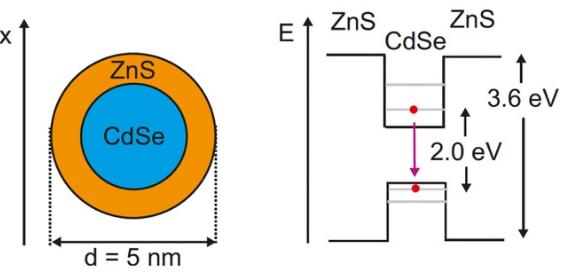
\includegraphics[width=0.5\textwidth]{Abb/ZnS_CdSe.png}
	\caption{Schematische Darstellung eines kolloidalen Typ-I CdSe/ZnS Quantenpunkts
   und seiner Energiestruktur \cite{anleitung}.}
	\label{fig:ZnS_CdSe}
\end{figure}
\noindent
Wird einem Nanokristall Energie in Form von Laserlicht zugeführt, so kann ein
Elektron aus dem Valenzband in das Leitungsband angehoben werden. Dabei hinterlässt
das Elektron ein Defekt, welches eine positive Ladung zugeschrieben werden kann.
Sowohl das Elektron als auch das Defektelektron relaxieren in einen energetisch
günstigeren Zustand nah der Bandlücke. Die überschüssige Energie wird dabei in
strahlungsloser Form an Phononen, Defekten, Störstellen oder anderen Ladungsträger
abgegeben. Da die Bandlücke zu groß ist, entsteht durch die Bindung von Elektron
und Defektelektron ein Exziton. Nach hinreichender Zeit kann es zu Rekombination
von Elektron und dem Defektelektron kommen, wodurch ein Photon mit der
Rekombinationsenergie abzüglich der Exzitonenbidungsenergie emittiert wird.
Es kommt zur Photolumineszenz. Ist die Energie des Laserlichtes größer als die
des CdSe-Kerns ($\SI{2,0}{\electronvolt}$) und kleiner als die der ZnS-Schale
($\SI{3,6}{\electronvolt}$), so entsteht in der ZnS-Schale zunächst ein
Elektron-Loch-Paar. Da es sich hier um einen Quantenpunkt Typ-I handelt, kann das
Elektron und das Defektelektron an die Bandlücke des CdSe-Kerns relaxieren.
In Abbildung \ref{fig:photoqp}(a) ist illustriert, wie der Quantenpunkt das
so entstandene Exziton einfängt. Befindet sich ein Elektron bereits im ZnS-Leitungsband,
wie in Abbildung \ref{fig:photoqp}(b) dargestellt, so ist von einem geladenen
Exziton die Rede. Ist die Laserleistung hoch, können sich auch Exzitonen auf höheren
Energieniveaus befinden, da eine Relaxation in ein tieferes Niveau nicht mehr
mögich ist (siehe dazu Abbildung \ref{fig:photoqp}(c)). Allerdings kann es bei
zu hohen Laserleistungen, und damit zu vermehrte Coulomb-Anziehung zwischen
den Elektron-Loch-Paaren, zur Veränderung der Bandstruktur kommen.

\begin{figure}[hbtp]
	\centering
	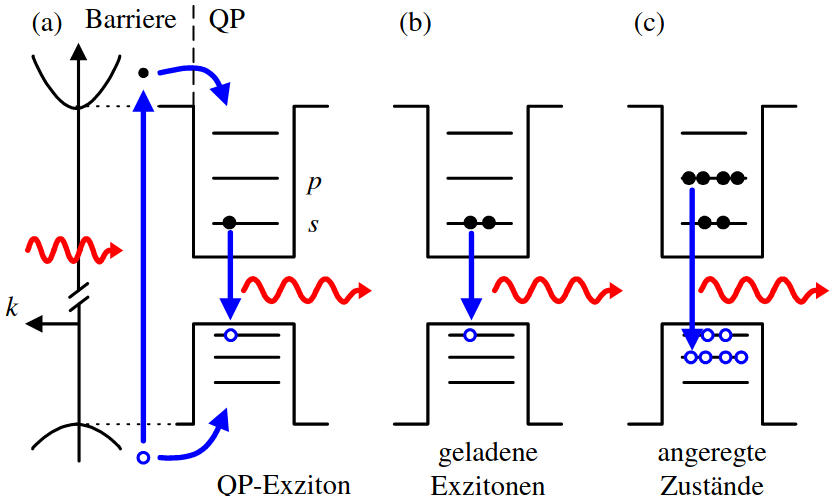
\includegraphics[width=0.8\textwidth]{Abb/photoqp.png}
	\caption{Schematische Darstellung eines kolloidalen Typ-I CdSe/ZnS Quantenpunkts
   und seiner Energiestruktur \cite{lars}.}
	\label{fig:photoqp}
\end{figure}
\noindent
Wie oben erwähnt, kann das Wachstum der Nanokristalle kontrolliert werden und
somit unterschiedlich große Bandlücken erzeugt werden. Dementsprechend lässt
sich auch die Energie des beim Rekombinieren entstehenden Photons, und damit auch
nach $E$ = $\frac{hc}{\lambda}$ die Wellenlänge $\lambda$ der Photolumineszenz wählen.
Dieses Verhalten ist in Abbildung \ref{fig:size} schematisch dargestellt.
\begin{figure}[hbtp]
	\centering
	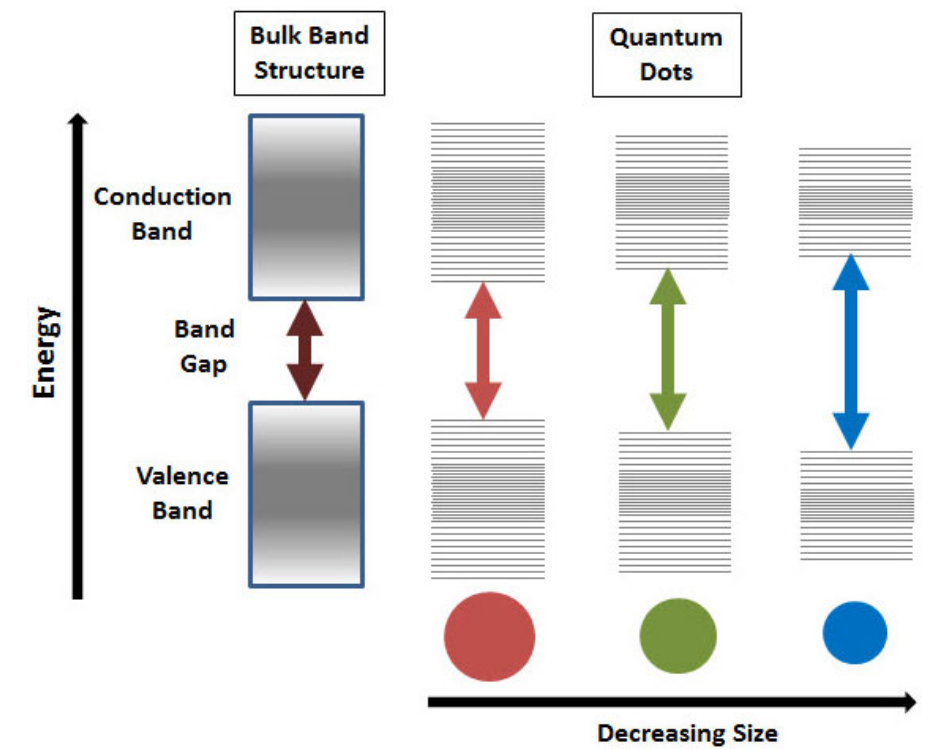
\includegraphics[width=0.6\textwidth]{Abb/size.png}
	\caption{Schematische Darstellung des Verhalten zwischen Nanokristallgröße und
  Wellenlänge $\lambda$ der Photolumineszenz\cite{size}.}
	\label{fig:size}
\end{figure}
\noindent
